\documentclass{article}
\usepackage[utf8]{inputenc}  % Поддержка UTF-8
\usepackage[T2A]{fontenc}   % Поддержка кириллицы
\usepackage{graphicx} % Поддержка изображений

\begin{document}

\title{Результаты обработки данных}
\author{Ваше имя}
\date{\today}

\maketitle

\section{Введение}

В этом документе представлены результаты обработки данных, визуализированные в виде графиков.

\section{Графики}

\begin{figure}[h!]
    \centering
    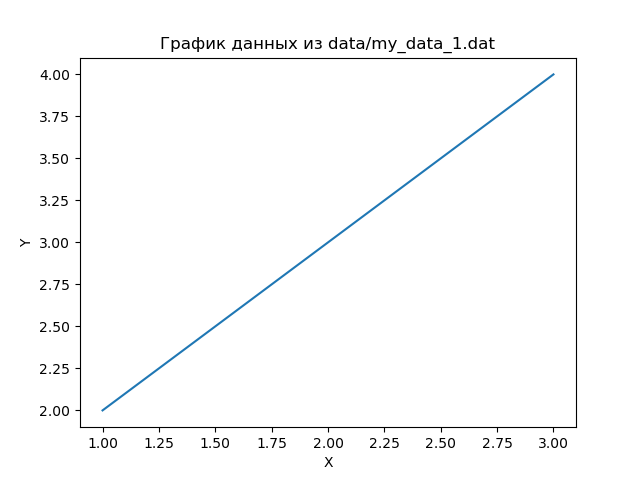
\includegraphics[width=0.8\textwidth]{figures/my_data_1.png}
    \caption{График случайных данных.}
    \label{fig:my_data_1}
\end{figure}

На рисунке \ref{fig:my_data_1} показаны случайные данные, сгенерированные и обработанные скриптом Python.

\begin{figure}[h!]
    \centering
    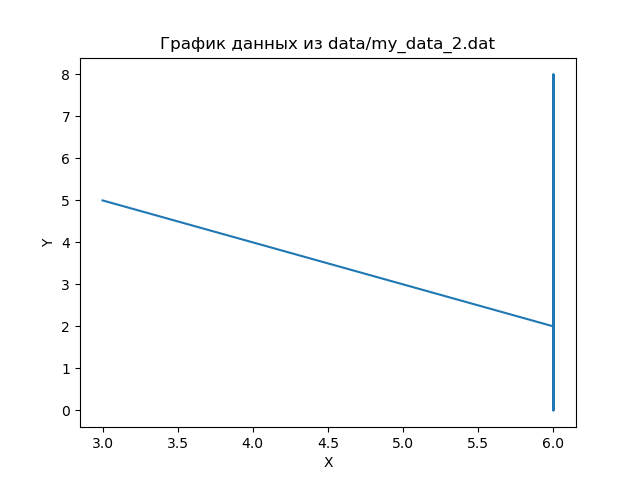
\includegraphics[width=0.8\textwidth]{figures/my_data_2.png}
    \caption{График случайных данных 2.}
    \label{fig:my_data_2}
\end{figure}

На рисунке \ref{fig:my_data_2} показаны случайные данные, сгенерированные и обработанные скриптом Python.

\end{document}
